\documentclass{article}

\usepackage{enumerate}
\usepackage{graphicx}
\usepackage{amsmath, amsthm, amssymb}

% Header macro
\def\AssignmentHeader#1#2#3{
  \title{
    % Assignment number
    % Provided in A sub n notation an standard english
    % using roman numerals.
    $A_{#1}$ \\ {\large Assignment \uppercase\expandafter{\romannumeral #1}} \\
    % Professor name and class.
    {\normalsize Prof. #2; #3}
  }
  \author{Connor Taffe}
}
% Configuration information
\AssignmentHeader{4}{Dr. P. Tang}{Computer Organization I}

\begin{document}
  \maketitle

  \begin{enumerate}
    % Describe the design, implementation and testing of the
    % task (b) of lab 11 as follows:

    % 1. Show the block diagram and function table of your ALU.
    \item{
      The block diagram is sketched and attached to this assignment.
      The function table in figure \ref{alutt} shows the output of the ALU in relation
      to the inputs $x$, $y$, and $z$ and the controls $S_{0-2}$. Note the $x$
      in the controls column is a placeholder for any value, and not the input
      $x$.
      \begin{figure}[h]
        \centering
        \begin{tabular}[h]{c c c | c}
          $S_{0}$ & $S_{1}$ & $S_{2}$ & ALU \\
          0 & 0 & 0 & $x+y$ \\
          0 & 0 & 1 & $x-y$ \\
          0 & 1 & 0 & $x\land y$ \\
          0 & 1 & 1 & $x$ \\
          1 & 0 & $x$ & $y$ \\
          1 & 1 & $x$ & $z'$ \\
        \end{tabular}
        \caption{\label{alutt} Truth table for ALU}
      \end{figure}
    }

    % 2. Show the internal circuits of your ALU.
    \item{
      Figure \ref{alucirc} shows the internal circuitry of the ALU.
      Notice that I have made a design descision alternate to that made
      in lecure five by bundling the negation of $z$ into the ALU. I understand
      that in a real situation, the Control Unit would have to coordinate the
      operations of more than one operational unit e.g. an FPU. For this reason,
      I will use an external not to create $z'$, to give the Control Unit something
      else to control.
      \begin{figure}[h]
        \centering
        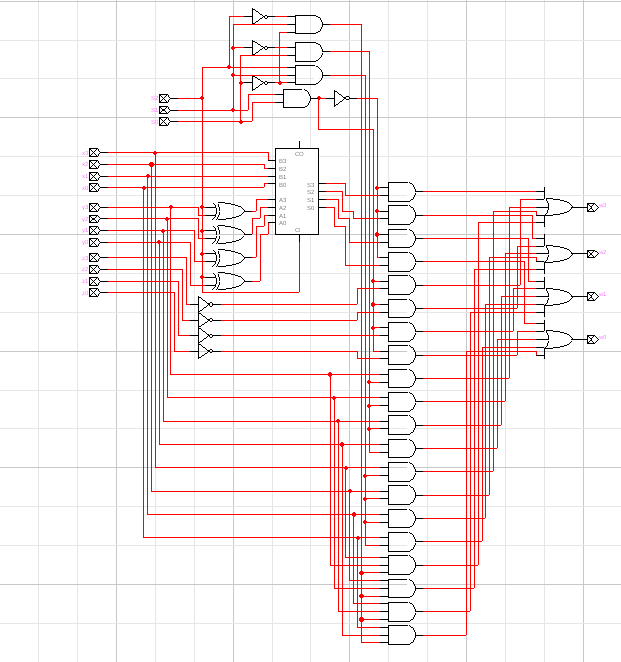
\includegraphics[width=300pt]{img/alu}
        \caption{\label{alucirc} Internal circuit of the ALU}
      \end{figure}
    }

    % 3. Show the block diagram of your datapath and
    % list all the control points.
    \item{
      The datapath diagram is sketched and attached to this assignment.
      The control points are $S_{0-2}$ for controlling the operation of
      the ALU, and loads for $x$, $y$, and $z$.
    }

    % 4. Show the circuit of you Datapath.
    \item{
      Figure \ref{dpcirc} shows the internal circuitry of the datapath.
      \begin{figure}[h]
        \centering
        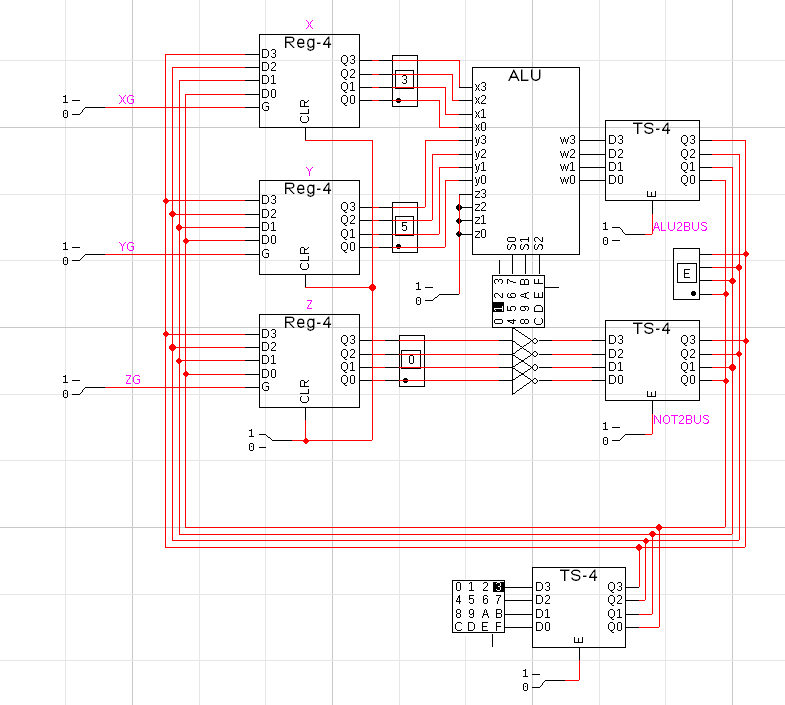
\includegraphics[width=300pt]{img/datapath}
        \caption{\label{dpcirc} Internal circuit of the datapath}
      \end{figure}
    }

    % 5. Show the control points activation table and derive
    % the Boolean equations of all control points.
    \item{
      Figure \ref{cptt} is the control point table which includes all six
      operations and their relevant control points settings.
      \begin{figure}[h]
        \centering
        \begin{tabular}[h]{c l | c c c c c c c c }
          && $S_{0}$ & $S_{1}$ & $S_{2}$ & load $x$ & load $y$ & load $z$ & ALU to bus & not to bus \\
          $\alpha$ & $x\leftarrow x+y$ & 0 & 0 & 0 & 1 & 0 & 0 & 1 & 0\\
          $\beta$ & $y\leftarrow x-y$ & 0 & 0 & 1 & 0 & 1 & 0 & 1 & 0 \\
          $\gamma$ & $x\leftarrow x\land y$ & 0 & 1 & 0 & 1 & 0 & 0 & 1 & 0 \\
          $\delta$ & $z\leftarrow x$ & 0 & 1 & 1 & 0 & 0 & 1 & 1 & 0 \\
          $\epsilon$ & $x\leftarrow y$ & 1 & 0 & 0 & 1 & 0 & 0 & 1 & 0 \\
          $\theta$ & $x\leftarrow z'$ & 1 & 1 & 0 & 1 & 0 & 0 & 0 & 1 \\
        \end{tabular}
        \caption{\label{cptt} Control Point table}
      \end{figure}

      \begin{figure}
        \begin{align}
          S_{0} &= \epsilon + \theta \\
          S_{1} &= \gamma + \delta + \theta \\
          S_{2} &= \beta + \delta \\
          \text{load $x$} &= \alpha + \gamma + \epsilon + \theta \\
          \text{load $y$} &= \beta \\
          \text{load $z$} &= \delta \\
          \text{ALU to bus} &= \alpha + \beta + \gamma + \delta + \epsilon \\
          \text{not to bus} &= \theta \\
        \end{align}
        \caption{\label{cpeq} Boolean equations for controls}
      \end{figure}
    }

    % 6. Show the internal circuit of your control unit.
    \item{
      Figure \ref{cucirc} shows the internal circuitry of the Control Unit.
      \begin{figure}[h]
        \centering
        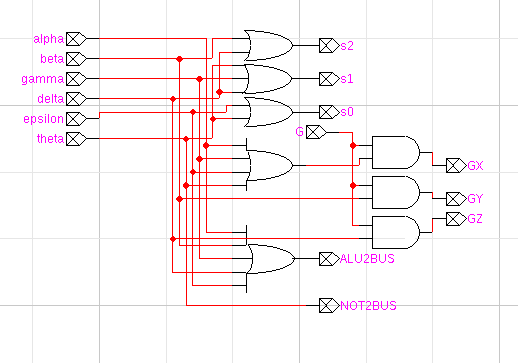
\includegraphics[width=300pt]{img/cu}
        \caption{\label{cucirc} Internal circuit of the control unit}
      \end{figure}
    }

    % 7. Testing your register transfer system under the
    % control of clock as follows:
    \item{
      \begin{enumerate}[(a)]

        % (a) Set the registers X, Y and Z to be hex 4, 1 and 7, respectively
        \item{
          I set the registers to the appropriate numbers. The testing
          circuit in the next question is photographed with those properties.
        }

        % (b) Show your testing circuit.
        \item{
          Figure \ref{tcirc} shows the testing circuit.
          \begin{figure}[h]
            \centering
            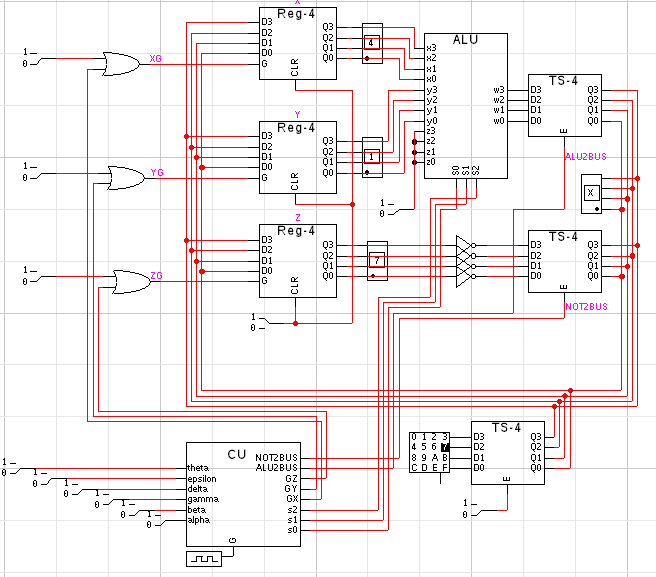
\includegraphics[width=300pt]{img/tcirc}
            \caption{\label{tcirc} Testing circuit}
          \end{figure}
        }

        % (c) Calculate the register value changes if we perform α, β, γ,
        % δ, ǫ and θ operations at 6 consecutive rising edges of G.
        \item{
          The calculations are shown in figure \ref{calc}.
          \begin{figure}
            \begin{align}
              x &\leftarrow 4 + 1 = 5 \\
              y &\leftarrow 5 - 1 = 4 \\
              x &\leftarrow 5 \land 4 = 4 \\
              z &\leftarrow 4 \\
              x &\leftarrow 4 \\
              x &\leftarrow 4' = 11 \\
              x &= 11 \\
              y &= 4 \\
              z &= 4 \\
            \end{align}
            \caption{\label{calc} Calculations of value changes.}
          \end{figure}
        }

        %(d) Show the waveform showing that the system performs α, β, γ,
        % δ, ǫ and θ, at 6 consecutive rising edges of G to confirm that
        % the system does make the register value changes as you calculated
        % in 7(c). You need to annotate the waveform to show these 6 changes.
        \item{
          Figure \ref{wave} waveform shows the testing. As you can see, the registers
          simulate with a fuzzy value after a few iterations. I have used those same
          registers before and they performed well. The circuit seems valid and the
          CU is making correct decisions. I also tested the ALU several times and
          it also seems to function properly. I have no idea what is causing the
          blurring. I have retried the simulation several times.
          Also the $g$ signal for $x$ is not shown properly as it is possibly
          labeled incorrectly. But you can see from the values propogating to
          it that it is functioning properly.
          \begin{figure}[h]
            \centering
            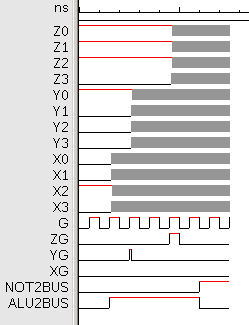
\includegraphics[width=150pt]{img/waveform}
            \caption{\label{wave} Waveform for circuit}
          \end{figure}
        }

      \end{enumerate}
    }
  \end{enumerate}

\end{document}
